% begin module closed-interval-method-ex
\begin{frame}
\begin{example}
Find the maximum and minimum values of the function $f(x) = -x^3 +2x^2+4x-5$ on the interval $\alert<handout:0| 9>{[1,3]}$.
\begin{columns}[c]
\column{.4\textwidth}
\psset{xunit=0.7cm, yunit=0.7cm}
\begin{pspicture}(-5, -5)(5,5) 
\tiny
\psframe*[linecolor=white](-5,-5)(5,5) 
\psaxes{<->}(0,0)(-0.5,-4.5)(4.5,4.5)
%Function formula: - ((x)^{3})+2 ((x)^{2})-5+4 (x) 
\uncover<11->{
\psFullDot{1}{0}
\rput[br] (1, 0.1){$(1,0)$} 
}
\uncover<13->{
\psFullDot{2}{3}
\rput[b] (2, 3.1){$(2,3)$} 
}
\uncover<15->{
\psFullDot{3}{-2}
\rput[bl] (3, -1.9){$(3,-2)$} 
}
\uncover<16->{
\rput[t](2,-3){$y=- x^{3}+2 x^{2}+4 x-5$} 
\psplot[linecolor=red, plotpoints=1000]{1}{3}{x 4 mul -5 add x 2 exp 2 mul add x 3 exp -1 mul add }
}
\end{pspicture} 
%\ \only<handout:0| -10>{%
%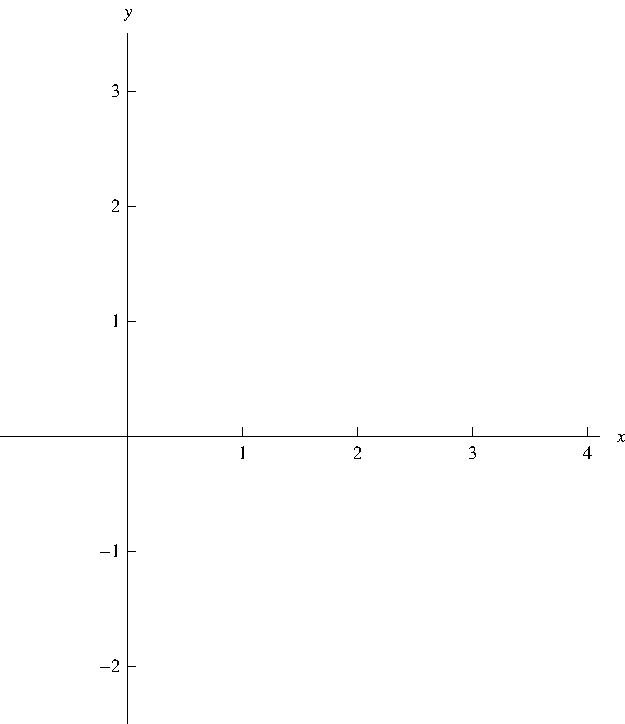
\includegraphics[width=5cm]{maxima-minima/pictures/04-01-ex8a.pdf}%
%}%
%\only<handout:0| 11-12>{%
%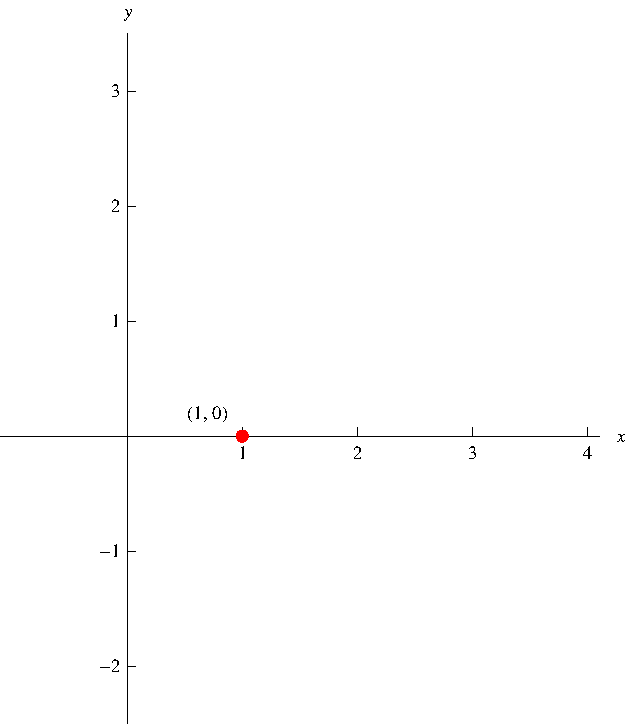
\includegraphics[width=5cm]{maxima-minima/pictures/04-01-ex8b.pdf}%
%}%
%\only<handout:0| 13-14>{%
%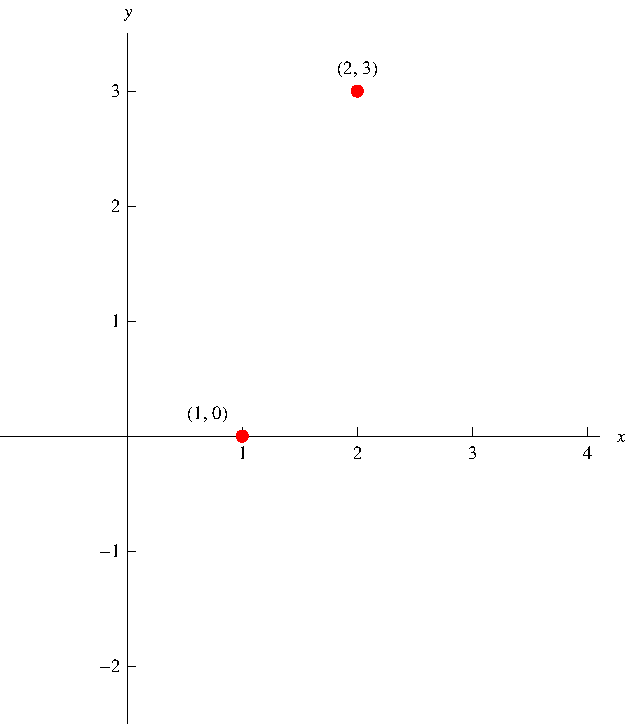
\includegraphics[width=5cm]{maxima-minima/pictures/04-01-ex8c.pdf}%
%}%
%\only<handout:0| 15>{%
%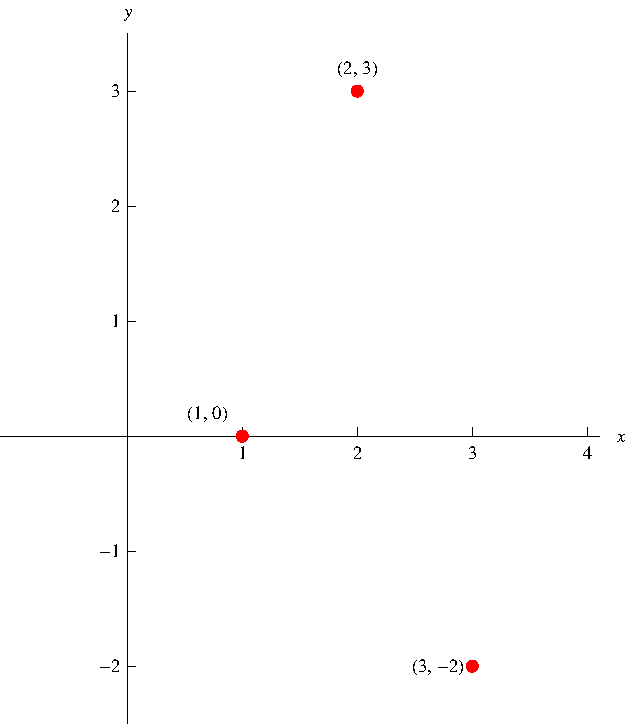
\includegraphics[width=5cm]{maxima-minima/pictures/04-01-ex8d.pdf}%
%}%
%\only<16->{%
%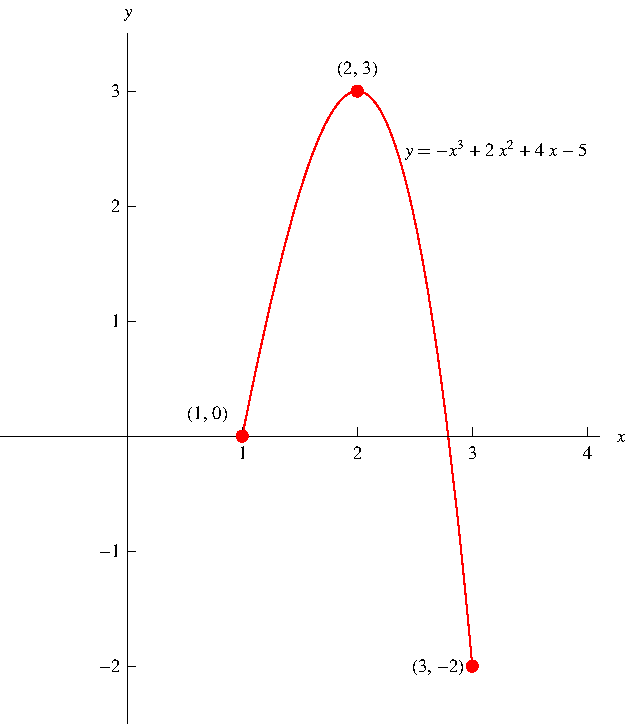
\includegraphics[width=5cm]{maxima-minima/pictures/04-01-ex8e.pdf}%
%}%
\column{.6\textwidth}
\abovedisplayskip=0pt
\belowdisplayskip=0pt
\abovedisplayshortskip=0pt
\belowdisplayshortskip=0pt
\begin{align*}
\uncover<2->{%
f'(x) %
}%
& \uncover<2->{ = } %
\uncover<2->{%
-3x^2 + 4x + 4%
}\\%
& \uncover<3->{ = } %
\uncover<3->{%
(-3x-2)(x-2)%
}%
\end{align*}
\uncover<4->{%
If $f'(x) = 0$, $x = -\frac{2}{3} \  \text{ or } \ \alert<handout:0| 7>{2}$.
}%

\uncover<5->{Need to check:}
\begin{enumerate}
\item<5-| alert@6-7>  The critical numbers of $f$ in $[a,b]$.
\item<5-| alert@8-9>  The endpoints $a$ and $b$.
\end{enumerate}
\[
\uncover<5->{%
\begin{array}{r|r}
x & f(x)\\
\hline
\uncover<9->{%
\alert<handout:0| 9-11>{1}
} &%
\uncover<11->{%
\alert<handout:0| 11>{0}
} \\%
\uncover<7->{%
\alert<handout:0| 7,12-13>{2}
} &%
\uncover<13->{%
\alert<handout:0| 7,12-13>{3}
} \\%
\uncover<9->{%
\alert<handout:0| 9,14-15>{3}
} &%
\uncover<15->{%
\alert<handout:0| 7,14-15>{-2}
} \\%
\end{array}
}%
\]
\end{columns}
\uncover<17->{%
\alert<handout:0| 17-18>{Absolute maximum: \uncover<18->{3.}}  \alert<handout:0| 19-20>{Absolute minimum: \uncover<20->{$-2$.}}
}%
\end{example}
\end{frame}
% end module closed-interval-method-ex
